\documentclass[12pt]{article}
\usepackage{graphicx,amssymb,amsmath,setspace,comment,verbatim,titling,pgf,lscape,color}
\usepackage[left=2cm,right=2cm,top=2.5cm,bottom=2cm]{geometry}
\usepackage[round]{natbib}
\usepackage{hyperref}
\usepackage{array}
\usepackage{bbm}
\usepackage{marginnote}
\usepackage[justification=centering]{caption}
%%\usepackage{breqn}
\newcommand{\pderiv}[2]{\frac{\partial#1}{\partial#2}}
%\usepackage{siunitx}
\newcolumntype{P}[1]{>{\raggedright\arraybackslash}p{#1}}
\hypersetup{colorlinks,%
						citecolor=black,%
						filecolor=black,%
						linkcolor=black,%
						urlcolor=blue,%
						}
\setstretch{1.5}

\setlength{\droptitle}{-50pt}

\begin{document}
\title{Decision Support and Health Insurance Choice}
\author{Ian McCarthy \& Evan Saltzman}
\date{March 18, 2021}
\maketitle

\vspace{-2ex}
\begin{abstract}
\noindent Abstract
\end{abstract}

\clearpage

\section{Introduction}
\label{sec:introduction}

Health insurance markets are unique in many respects, not least of which is the increasing complexity of choosing an optimal health insurance plan. Such complexity has been well-documented in studies of health insurance choice in the Medicare Advantage market \citep{abaluck2011, ketcham2012, gruber2017}. One way to reduce the burden of this complexity is to provide professional decision support through private insurance agents or public assistance programs, both of which are available in the California health insurance exchanges created under the Affordable Care Act (ACA). In this paper, we examine the role of this decision assistance on health insurance plan choice and its implications for consumer welfare.

\section{Background and Motivation}
\label{sec:background-and-motivation}

Discussion of poor decision making in health insurance and role of experts.

\section{Data}
\label{sec:data}

Our final dataset consists of 3,212,732 household/year observations from the California health insurance exhanges from 2014 to 2019. Our data include a variety of household characteristics, plan choices and plan characteristics, and information on the type of decision assistance used by the enrollee (if any). From these data, we can identify each household's set of possible health insurance plans, and we employ premium and cost sharing subsidy formulas to calculate health insurance costs for each possible plan for each household

\section{Methods}
\label{sec:methods}

Our overarching goal is to estimate the effect of decision assistance on health insurance decisions; however, there are many ways of measuring ``health insurance decisions''. One approach is to estimate demand for health insurance in a traditional discrete choice framework. This would allow us to quantify individuals' willingness to pay for decision assistance as well as the effect of decision assistance on choice probabilities. Another approach is to focus specifically on ``dominated choices'', which are relatively clearly defined and observable in our empirical context. This latter approach lacks the richness of the discrete choice demand framework but benefits from a focus on a specific outcome of obvious policy and welfare relevance. We consider both approaches in our analysis, as detailed in the remainder of this section.

\subsection{Discrete Choice Framework}
\label{subsec:discrete-choice-framework}

We model health insurance purchasing with a nested logit discrete choice model, as in \cite{saltzman2019}, and we derive estimates of the effect of decision assistance by embedding this discrete choice model into a standard potential outcomes framework.

For our discrete choice model, we assume that household \(i\) chooses the plan \(j\) that maximizes their utility,
\begin{equation}
u_{ij} = \alpha_{i}p_{ij} + \beta x_{j} + \gamma d_{i} + \xi_{j} + \varepsilon_{ij}, \label{eq:utility}
\end{equation}
where \(p_{ij}\) denotes the premium for plan \(j\), \(x_{j}\) denotes a vector of product characteristics, \(d_{i}\) denotes a vector of household characteristics, \(\xi_{j}\) captures unobserved product characteristics, and \(\varepsilon_{ij}\) is an error term assumed to follow a type I extreme value distribution. We allow for heterogenities in price elasticities across households by parameterizing \(\alpha_{i}\) in Equation \eqref{eq:utility}, \[\alpha_{i} = \alpha + \theta d_{i}.\] In our estimation, this amounts to including a full set of interactions between \(d_{i}\) and \(p_{ij}\).

\subsection{Dominated Choices}
\label{subsec:dominated-choices}

As a complementary empirical analysis, we identify specific instances in which the observed plan choice is dominated by some other plan in an individual's choice set, and we estimate the effects of decision assistance on the probability of making such a choice. For example, Gold and Platinum tier plans are dominated for any household that is eligible for cost-sharing subsidies and with incomes below 150\% of the federal poverty level. We estimate the effect of decision assistance on dominated choices with a linear probability model, allowing for year, insurer, and region fixed effects.

\section{Results}
\label{sec:results}

Our nested logit models establish strong evidence that decision assistance matters for insurance choice. Turning specifically to dominated choices, our baseline results suggest that individuals with decision assistance are 1.4 percentage points less likely to make a dominated choice. On a base of 2.8\%, this reflects a 50\% decrease in the probability of making a dominated choice.

We also find evidence fo heterogeneities in the effects of different forms of decision assistance. In particular, we find that individuals using publicly provided decision assistance are 1.09 percentage points less likely to select a dominated plan, while individuals using a private insurance agent are 1.54 percentage points less likely to select a dominated plan.

\section{Conclusion}
\label{sec:conclusion}

Our current results provide strong evidence that decision assistance has a significant and economically meaningful effect on health insurance plan choice. In terms of dominated choices, our early results suggest that this change in decision-making is welfare improving, and we continue to explore other measures of choice dominance to further confirm this result.

In future work, our identification strategy will exploit the Trump administration's removal of cost-sharing subisidies from the exchanges in 2018 and the subsequent response from insurers to increase premiums on their silver plans (``silver loading''). This response significantly changed the prevalence of dominated choices in each household's choice set, and in this way, the removal of the cost-sharing subsidies offers an exogenous change to the set of dominated plans available to each household.

We are also extending our analysis of the differential effects between public decision support versus assistance from private insurance agents/brokers. This analysis will determine whether insurance brokers are more likely to steer patients into plans offered by the sponsoring insurer.

\pagebreak
\bibliographystyle{authordate1}
\bibliography{BibTeX_Library}

\clearpage
\newpage


\section*{Tables and Figures}

\begin{figure}[htb]\caption{Count of Enrollees in California Exchange}
\centering
 		\hspace*{-1cm}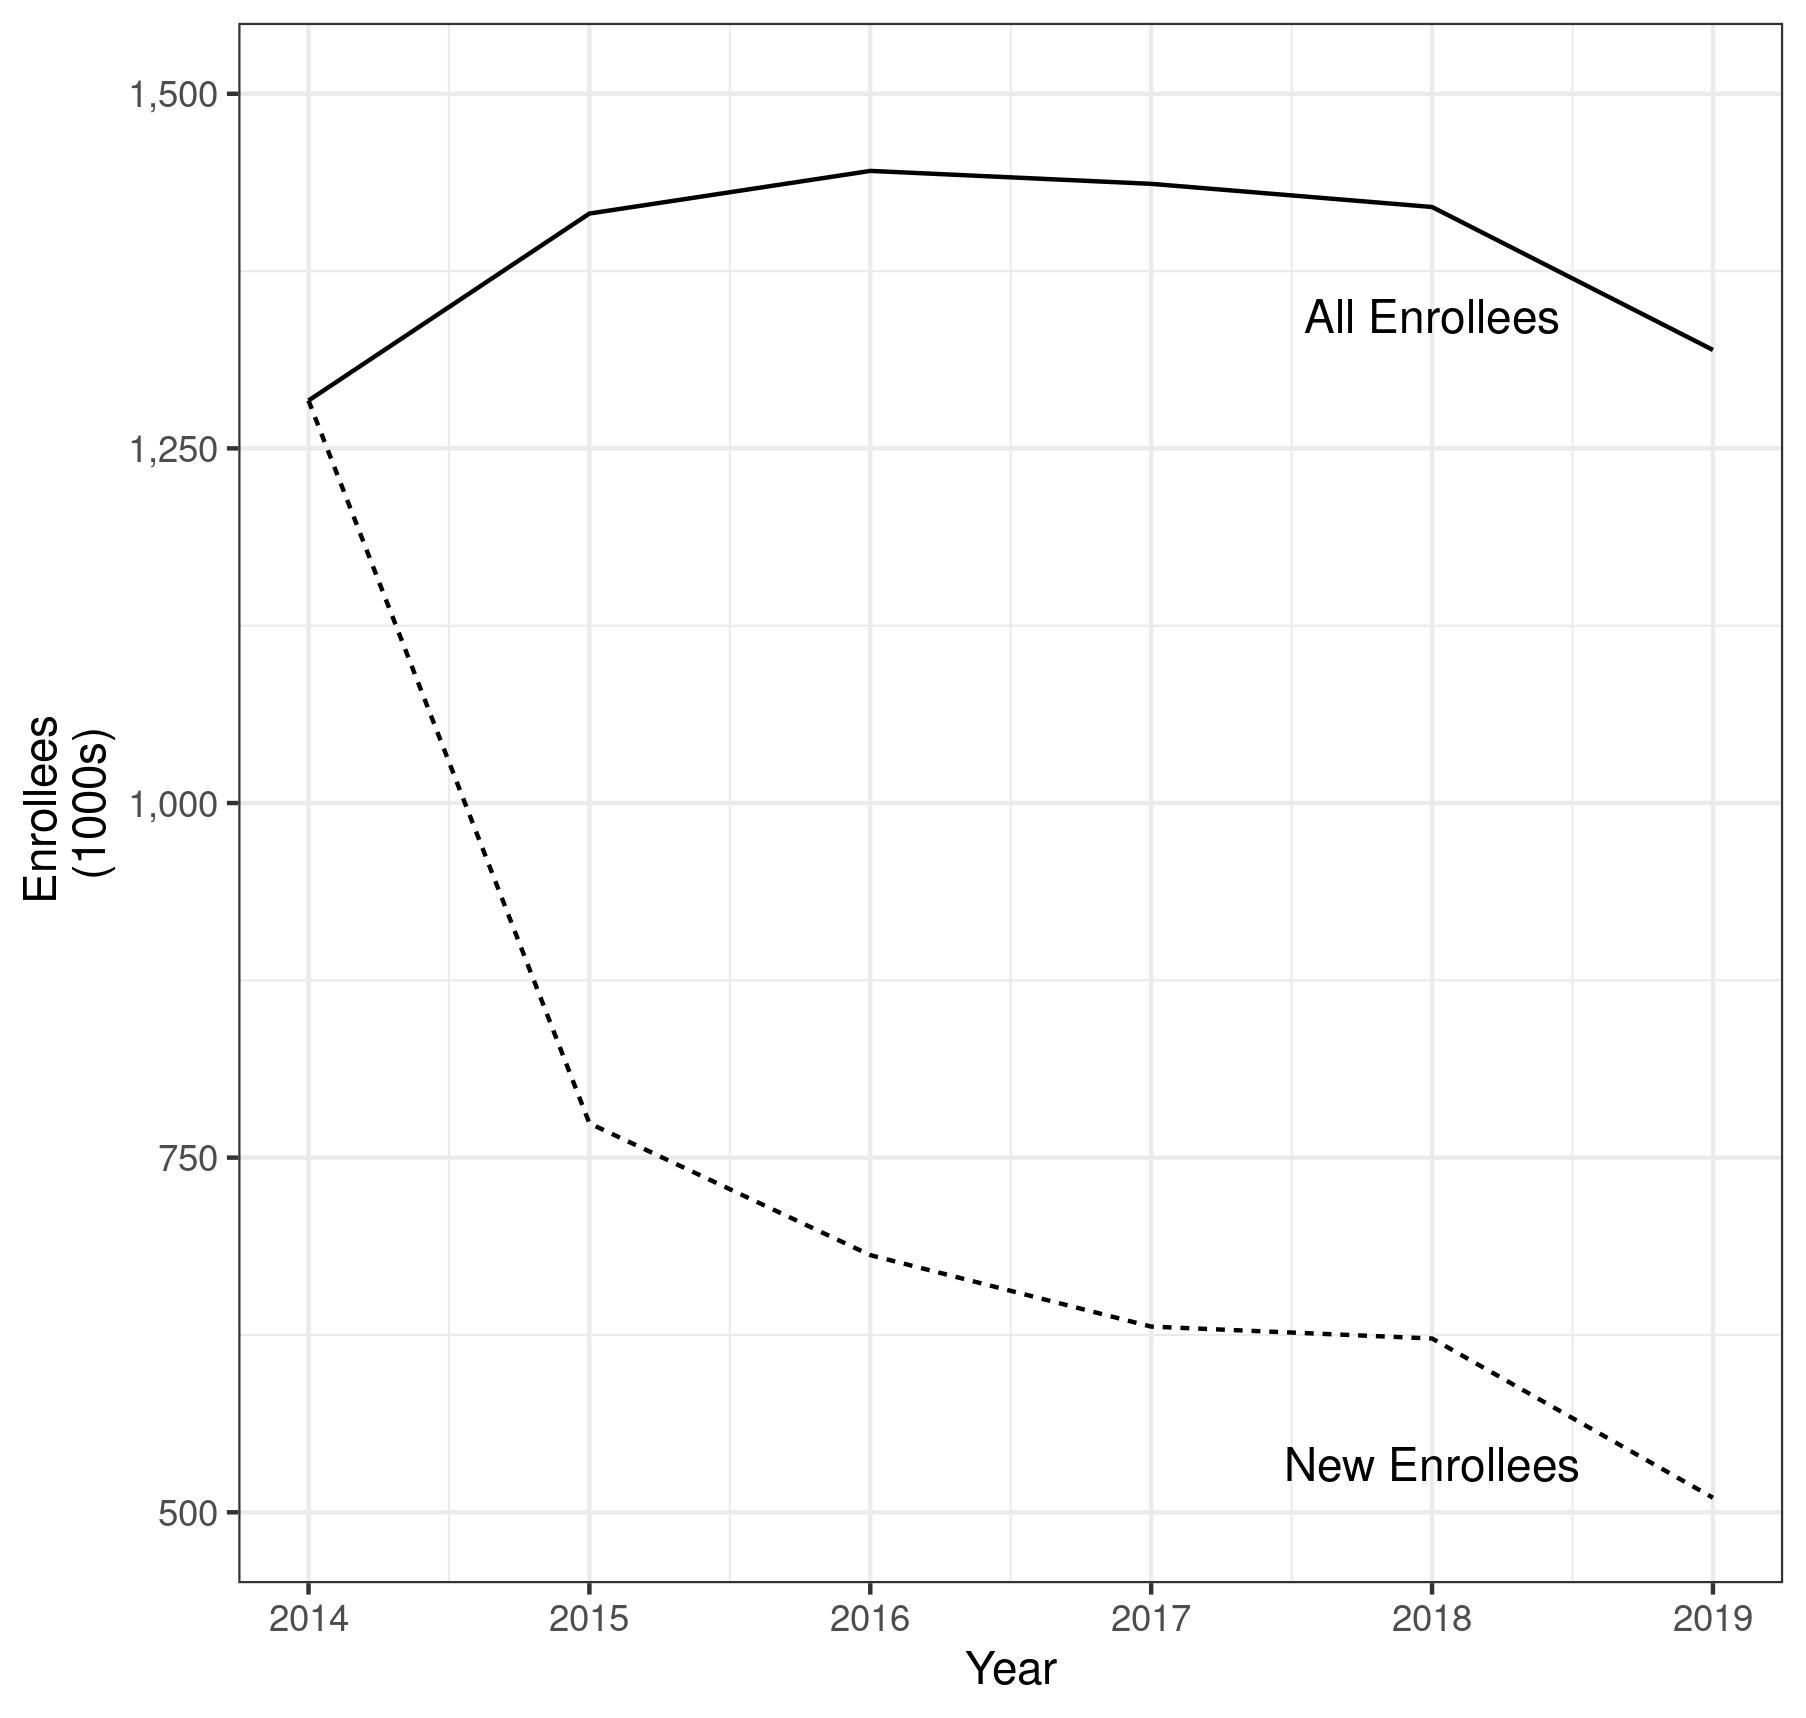
\includegraphics[scale=.7]{figures/enrollee_count.png}
 		\begin{minipage}{\textwidth}
		\bigskip
			\footnotesize \textsc{Notes:} The coefficients for high ratings are shown with circles, those for middle ratings are shown with triangles, and no reviews are shown with diamonds. The main results are designated in blue along with an indicator for specification ``Main". Various specifications and required minimum number of reviews are also indicated. 
 		\end{minipage}
 		\label{figure:SpecCurve}
 \end{figure}

\end{document}
